%----------------------------------------------------------------
%
%  File    :  set_up.tex
%
%  Authors :  David Lechner, FH Campus Wien, Austria
%
%  Created :  10 Oct 2019
%
%  Changed :  10 Oct 2019
%
%----------------------------------------------------------------


\chapter{Versuchsaufbau}
\label{chap:set_up}

Dieses Kapitel geht auf den Versuchsaufbau des Systems ein. Anfangs werden die zur Verfügung stehenden Daten beschrieben und wie diese für \textit{Machine Learning} vorverarbeitet werden. Danach wird der erste Versuch gezeigt, wie mit ML und den Daten eine Fahreridentifizierung durchgeführt werden kann. Für jegliche Programmieranwendung wurde \textit{Python} aufgrund der zahlreichen Module und des vorhandenen \textit{Know-Hows} verwendet.

\section{Trainingsdaten}
\label{sec:data_description}

Die Daten, welche für die Masterarbeit vorliegen, wurden dankenswerterweise von einem Kollegen bereitgestellt, der diese im Zuge einer Studie über einen längeren Zeitraum aufgezeichnet hat. Dabei handelt es sich um CAN-Nachrichten, aufgenommen in neun Fahrzeugen (VW Golf 7, keine näheren Informationen) während des Fahrens. Es wurde sichergestellt, dass jeweils nur eine Person hinter dem Lenkrad gesessen ist. Ein Boardcomputer mit Internetkonnektivität (ALEN, siehe \ref{sec:ccu}) im Fahrerraum ist für die Aufzeichnung verwendet worden. Das \textit{Embedded-Device} ist über zwei CAN-Bus Schnittstellen mit der Fahrwerks-Linie (F-CAN) und der Komfort-Linie (K-CAN) verbunden und kann somit alle Nachrichten in fast-Echtzeit vom Bus mitlesen. Dabei ist aber sichergestellt, dass es nicht möglich ist, auch Nachrichten senden zu können, da dies bei einer Fehlfunktion zu einem Unfall führen und Insassen gefährden könnte. Die Nachrichten werden nach dem Empfangen mit einem synchronisierten Zeitstempel, aufgelöst in Nanosekunden, versehen und in eine MDF Datei mit den Metadaten von der entsprechenden DBC-Datenbank gespeichert. Eine Datei enthält jeweils Messdaten über eine Dauer von einer Minute. Danach wurde die Datei temporär auf einer Festplatte gespeichert und auf einen File-Server über eine LTE-Funkverbindung hochgeladen. Um sie über alle Fahrzeuge hinweg eindeutig zuordnen zu können, wurde eine Fahrzeugidentifikationsnummer dem Dateinamen angehängt.

In einer Datei sind 46 verschiedene Signale der beiden CAN-Busse enthalten. Tablle \ref{tab:can_signals} listet die meisten davon. Jene, die sich vorrausichtlich nicht für die Analyse eignen, wie z.B. die Innentemperatur oder der Status des Standlichts, sind ausgenommen. Für die komplette Liste siehe Anhang. Pro Datei sind durchschnittlich 100000 Messwerte vorhanden, daraus ergeben sich bei einer Anzahl von 10359 Dateien über eine Milliarde Messpunkte. Die folgende Liste gibt einen Einblick über die vorhandenen Daten.
% TODO: Anhang mit kompletter Liste

\begin{itemize}
  \item Anzahl Fahrer: 9
  \item Datengröße (MDF): 4.9 GB
  \item $\diameter$ Fahrtenanzahl: 46
  \item Fahrtenanzahl insgesamt: 421
  \item $\diameter$ Fahrzeit pro Fahrer pro Fahrt: 23 Minuten
  \item $\diameter$ Fahrzeit pro Fahrer: 18 Stunden
  \item Fahrzeit insgesamt: 165 Stunden
  \item $\diameter$ Gefahrene Kilometer: 1046
  \item Gefahrene Kilometer insgesamt: 9411
  \item Zeitraum: 13.07.2019 - 21.08.2019
  \item Geographischer Bereich: Stuttgart, Deutschland
\end{itemize}

Die Fahrrouten sind nicht speziell beschränkt, sondern sind von Fahrzeug zu Fahrzeug unterschiedlich, was die Fahrtdauer, Tageszeit und Route betrifft. Dadurch sind die Messdaten in sehr realen Bedingungen aufgenommen worden.

\begin{table*}[htbp]
	\centering
  \begin{tabular}{|l|l|l|l|l|}
  \hline
  Signalname & CAN-Bus & Beschreibung & Einheit & Wertbeschr. \\
  \hline
  LWI\_Lenkradwinkel & F-CAN & Lenkradwinkel & Grad & - \\
  LWI\_Lenkradw\_Geschw & F-CAN & \shortstack{Lenkradwinkel- \\ Geschwindigkeit} & Winkelsekunde & - \\
  ESP\_Fahrer\_bremst & F-CAN & Bremspedal betätigt & Boolean & \shortstack{0: nicht betätigt \\ 1: betätigt} \\
  ESP\_Bremsdruck & F-CAN & Bremsdruck & Bar & - \\
  MO\_Fahrpedalrohwert\_01 & F-CAN & Fahrpedalposition & - & - \\
  MO\_Kuppl\_schalter & F-CAN & Kupplung betätigt & Boolean & \shortstack{0: nicht betätigt \\ 1: betätigt} \\
  MO\_Drehzahl\_01 & F-CAN & Motordrehzahl & rpm & - \\
  KBI\_Tankfuellstand\_Prozent & F-CAN & Tankfüllstand & \% & - \\
  KBI\_Kilometerstand & F-CAN & Kilometerstand & km & - \\
  MO\_Gangposition & F-CAN & Gangposition & - & \shortstack{1: 1. Gang oder \\ Rückwärtsgang \\ 2-6: 2. - 6. Gang} \\
  ESP\_VL\_Radgeschw\_02 & F-CAN & \shortstack{Geschwindigkeit \\ Rad links vorne} & km/h & - \\
  ESP\_VR\_Radgeschw\_02 & F-CAN & \shortstack{Geschwindigkeit \\ Rad rechts vornen} & km/h & - \\
  ESP\_HL\_Radgeschw\_02 & F-CAN & \shortstack{Geschwindigkeit \\ Rad links hinten} & km/h & - \\
  ESP\_HR\_Radgeschw\_02 & F-CAN & \shortstack{Geschwindigkeit \\ Rad rechts hinten} & km/h & - \\
  ESP\_v\_Signal & F-CAN & \shortstack{Durchschnittliche \\ Radgeschwindigkeit} & km/h & - \\
  ESP\_HL\_Fahrtrichtung & F-CAN & \shortstack{Fahrtrichtung \\ Rad links hinten} & - & \multirow{2}{*}{\shortstack{0: Vorwärts \\ 1: Rückwärts}} \\
  ESP\_HL\_Fahrtrichtung & F-CAN & \shortstack{Fahrtrichtung \\ Rad links hinten} & - & \\
  ESP\_Laengsbeschl & F-CAN & Längsbeschleunigung & m/s\textsuperscript{2} & - \\
  ESP\_Querbeschleunigung & F-CAN & Querbeschleunigung & m/s\textsuperscript{2} & - \\
  ESP\_Gierrate & F-CAN & Gierrate & \shortstack{Grad pro \\ Sekunde} & - \\
  Wischer\_vorne\_aktiv & K-CAN & Wischer vorne aktiv & Boolean & \multirow{3}{*}{\shortstack{0: nicht aktiv \\ 1: aktiv}} \\
  BH\_Blinker\_li & K-CAN & Blinker links aktiv & Boolean & \\
  BH\_Blinker\_re & K-CAN & Blinker rechts aktiv & Boolean & \\
  \hline
  \end{tabular}
	\caption{Signalbeschreibung}
	\label{tab:can_signals}
\end{table*}

Je nach Steuergerät und Nachrichtentyp ist die Signalhäufigkeit unterschiedlich. Zum Beispiel sendet das Lenkrad- und Motorsteuergerät mit der gleichen Frequenz – nämlich 100-mal in der Sekunde. Andere jedoch, wie das Getriebesteuergerät, nur mit einer Frequenz von 10Hz. Abbildung \ref{fig:signal_freq} zeigt die Häufigkeit einiger Signale. Alle nicht-gelisteten haben entweder eine Frequenz von 10, 50 oder 100Hz.

\begin{figure}[htbp]
	\centering
		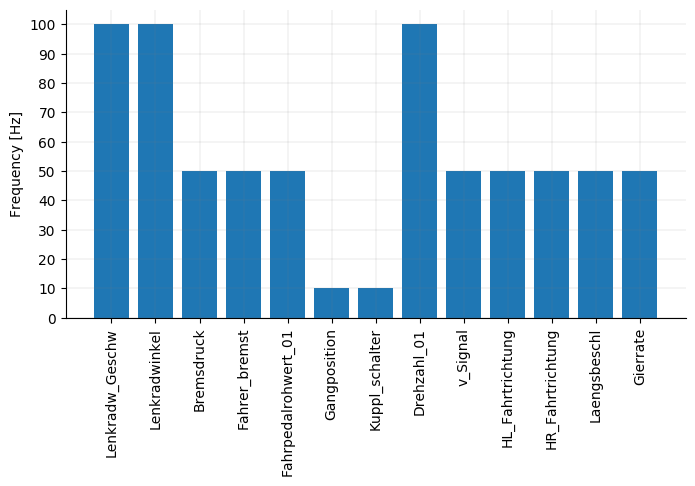
\includegraphics[width=.7\textwidth]{images/signal_frequences.png}
	\caption{Signalhäufigkeiten}
	\label{fig:signal_freq}
\end{figure}

\section{Datenvorbearbeitung}
\label{sec:data_preprocessing}

Werden alle Signale eliminiert, welche nicht unmittelbar vom Fahrer beeinflusst werden und so auch keine Individualität aufweisen, ergibt sich eine Anzahl von 14 verschiedenen Signalen. Das Einschalten des Blinkers oder des Fernlichtes lässt nicht direkt auf den Lenker schließen, da es vielmehr von der Umgebung - Kreuzung oder Einbruch der Dunkelheit - abhängig ist. Die Wahl des Ganges in einer Kurve jedoch schon, siehe Kapitel \ref{sec:overview}. Diese 13 Signale (später auch als \textit{Features} bezeichnet) sind:

\textit{Bremsdruck}, \textit{Gangposition}, \textit{Geschwindigkeit}, \textit{Motordrehzahl}, \textit{Fahrpedalrohwert}, \textit{Längsbeschleunigung}, \textit{Querbeschleunigung}, \textit{Lenkradwinkel}, \textit{Gierrate}, \textit{Bremspedal betätigt}, \textit{Lenkradgeschwindigkeit}, \textit{Kupplung betätigt}, \textit{Fahrtrichtung}

Für jede \textit{Machine Learning} Anwendung ist es ausschlaggebend, dass die Daten durchgängig strukturiert und einheitlich sind. Das Ziel ist also, Datensätze zu bekommen, wo jedes Signal einen Wert hat und einer Fahrerin zugeordnet ist. Da sich die Häufigkeit jedoch unterscheidet, müssen die Signale angeglichen werden, um so eine gemeinsame Frequenz zu bekommen. Laut dem Paper von M. Enev et al. liegt der Wert mit dem besten Endresultat bei 0.5Hz.\footnote{\cite{Enev2016}} Aus allen Signalpunkten wurde daher der Durchschnitt über zwei Sekunden berechnet. Dadurch gehen aber auch Informationen verloren, wie zum Beispiel eine kurze Beschleunigung nach einer Kurve. Um dies zu erhalten, wird auch der Maximal- sowie der Minimalwert mitgenommen. Weiters kommt noch der Median und die Standardabweichung hinzu. Daraus ergibt sich ein Datenset aus 65 Signalen und die Fahreridentifikation. Abbildung \ref{fig:dataset} zeigt einen Auszug der Daten.

\begin{figure}[htbp]
	\centering
		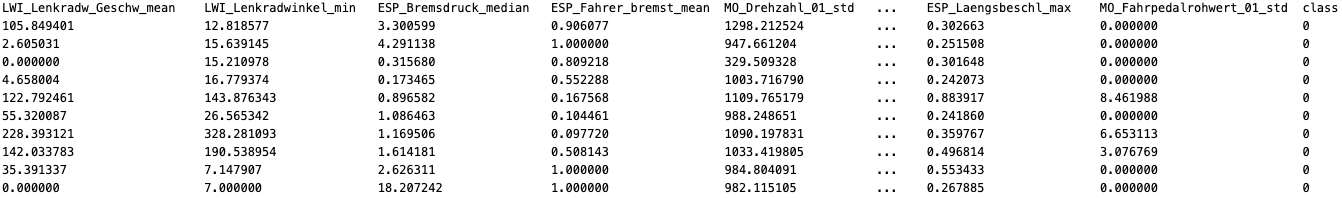
\includegraphics[width=\textwidth]{images/dataset.png}
	\caption{Auszug aus Datenset}
	\label{fig:dataset}
\end{figure}

Für eine einfachere Weiterverarbeitung und etwaige Manipulationen müssen die Daten zwischengespeichert werden. Hierfür bietet sich das Format \textit{Hierarchical Data Format version 5} (HDF5) an, welches der de facto Standard für die Speicherung von großen Datensets in \textit{Python} ist. Es bietet sowohl ein schnelles Einlesen und Schreiben von Daten, als auch die Anwendung von Operationen auf ganze Datenreihen, wie beispielsweise die Berechnung des Durchschnitts oder die Bestimmung der Standardabweichung.\cite{Collete2013}

\section{Scikit-Learn}
\label{sec:sk_learn}

Die Programmiersprache \textit{Python} erfreut sich in den letzten Jahren an einer immer mehr werdenden Popularität. Dank der einfachen Syntax und einer Vielzahl an wissenschaftlichen Bibliotheken ist sie auch besonders für Datenanalyse interessant. Das Modul \textit{Scikit-Learn} \cite{scikit-learn} nützt diese Umgebung und bietet Implementierungen der aktuellsten \textit{Machine Learning} Algorithmen an. Es ist daher eine Antwort auf den wachsenden Bedarf an statistischer Datenanalyse vor allem in nicht wissenschaftlichen Bereichen wie der Software- und Webentwicklung. \textit{Scikit-Learn} gilt als performant und intuitiv, da sie grundlegende Strukturen und Module von \textit{Python} verwendet. Darunter zählen \textit{Numpy}, \textit{Scipy} und \textit{Cython}. Des Weiteren werden auch sehr wenig andere externe Abhängigkeiten benötigt, was zusätzliche Performance bringt.

\section{Erster Versuch}

Als erster Schritt wurde der \textit{Random Forest} Algorithmus mit Standardwerten (siehe weiter unten) auf Messdaten angewendet, um zu validieren, dass eine Identifikation überhaupt mit den vorhanden Daten möglich ist. Hierfür wurden aus den gesamten Daten zufällige 20 Minuten Fahrtzeit pro Fahrer extrahiert, wobei der jeweils erste Datensatz der Beginn einer Fahrt ist. Laut Miro Enev et al. \cite{Enev2016} werden zwischen zehn und 15 Minuten Trainingszeit benötigt, um eine Identifikationsgenauigkeit von über 90\% zu erreichen. Da die Forscher mehr Daten zur Verfügung hatten, wurde die Zeit um fünf Minuten verlängert. Die neun (9 Fahrer) Datensets wurden dann zu einem zusammengefügt, vermischt und in die \textit{Features} beziehungsweise die Fahrerkennung (\textit{class}) aufgeteilt. Daraus sind zufällige sechs Minuten (30\%) entfernt worden, welche später zum Testen des \textit{Models} verwendet werden. Das Listing \ref{lst:rf_first_try} zeigt den Programmcode in \textit{Python}.

\begin{lstlisting}[frame=lines, caption=Erster Versuch mit \textit{Random Forest}, captionpos=b, label = lst:rf_first_try, numbers=left, language=Python, showstringspaces=false, basicstyle=\footnotesize]
import os
import sys
import pandas as pd
from sklearn.utils import shuffle
from sklearn.model_selection import train_test_split
from sklearn.ensemble import RandomForestClassifier
from sklearn import metrics

hdf5_input = sys.argv[1]
signals = ['can0_LWI_Lenkradw_Geschw_mean', 'can0_LWI_Lenkradwinkel_mean', ...]
frames = []
for file in os.listdir(hdf5_input):
  data = pd.read_hdf(os.path.join(hdf5_input, file))
  frames.append(data)

result = pd.concat(frames, sort=False)
result = shuffle(result)
X = result[signals]
Y = result['class']
X_train, X_test, Y_train, Y_test = train_test_split(X, Y, test_size=0.3)

clf = RandomForestClassifier()
clf.fit(X_train, Y_train)
Y_pred = clf.predict(X_test)
accuracy = metrics.accuracy_score(Y_test, Y_pred)

print('Accuracy:' , accuracy)
\end{lstlisting}

Dabei ist eine Identifikationsrate von 85\% Prozent erzielt worden. Das bedeutet, dass das ML-\textit{Model} über 150 Datenreihen aus 180 pro Fahrer ($6[min] * 60 * 0,5Hz = 180$) den tatsächlichen Fahrern zuordnen konnte und bestätigt eine Identifizierung mit den vorhanden Daten. Bei einem erneuten Versuch war die Wahrscheinlichkeit fast 91\% und beim dritten unter 83\%, mit jeweils anderen zufälligen Daten. Die Ergebnisse von weiteren Durchläufen sind in der Abbildung \ref{fig:rf_tries} ersichtlich. Die erste Schlussfolgerung daraus ist, dass eine Identifikation mit den Daten und der Methode möglich ist. Weiters hat die Auswahl der Daten einen erheblichen Einfluss auf das Ergebnis. So war die geringste Wahrscheinlichkeit 78,66\% und die höchste 92,53\%. Im Mittel sind 86,4\% erzielt worden.

\begin{figure}[htbp]
	\centering
		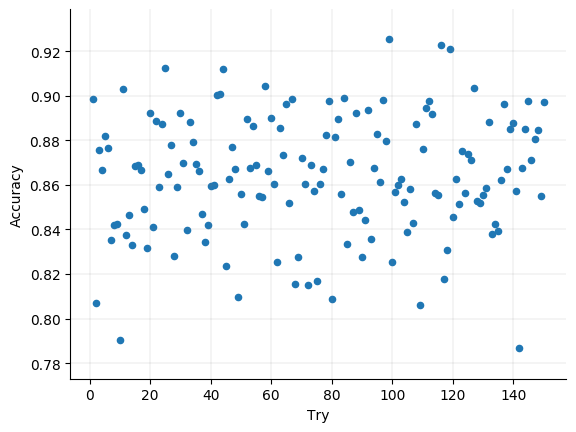
\includegraphics[width=0.7\textwidth]{images/rf_accuracy.png}
	\caption{\textit{Random Forest} Versuche}
	\label{fig:rf_tries}
\end{figure}
